\documentclass{article}
\usepackage{geometry}
\usepackage{graphicx}
\usepackage{booktabs}
\usepackage{float}
\usepackage{array}
\usepackage{hyperref}
\usepackage[super,sort&compress]{cite}

\hypersetup{
    colorlinks=true,
    linkcolor=black,
    citecolor=black,
    urlcolor=blue
}
\newcolumntype{C}{>{\centering\arraybackslash}c}
\title{SPLASH}
\author{Iasonas Lamprinidis, Vasileios Zoidis, Ioannis Michalainas, Savvas Tzanetis}
\date{May-June 2025}

\begin{document}

\maketitle
\begin{center}
  \textbf{Repository:} \\
  \href{https://github.com/ioannisam/SPLASH}{github.com/ioannisam/SPLASH}
\end{center}
\bigskip
\begin{abstract}
    \centering{SPLASH - Sea Parameter Logging And Sensor Hub. \newline A brief overview of the project: goals, key features and overall system architecture.}
\end{abstract}
\tableofcontents
\clearpage

\newgeometry{top=1.5cm, bottom=1.5cm, right=1.5cm, left=1.5cm}
\section{Introduction}
This project implements a \textit{remote weather station}. The premise is to use multiple Arduino devices to create a network of data nodes. These nodes will monitor temperature, pressure and estimated wave shore impact/height at sea level. The collected data will then be displayed on a web application for fishermen, researchers, or hobbyists to use.
    
    \subsection{Motivation and Objectives}

    The primary motivation for this project is to enable \textbf{cost-effective}, \textbf{modular} \textbf{remote monitoring} of maritime weather conditions using low-power Arduino nodes. Real-time insights into \textit{temperature}, \textit{atmospheric pressure} and \textit{wave activity} (approximated via accelerometer data) are crucial for coastal monitoring, fishing safety and climate research.
    
    \vspace{0.5cm}
    \textbf{Objectives}:
    \begin{itemize}
        \item Design a distributed sensor node that gathers environmental data.
        \item Implement wireless communication between sensor and receiver using RF modules.
        \item Display gathered information on a centralized platform.
        \item Optimize energy use through staggered data transmission and low-power components.
    \end{itemize}
    
    \subsection{Report Structure}
    This report's structure mimics the workflow of our app. We will be explaining from the bottom up the architecture, design choices and development stages of our project.

    \begin{figure} [h]
        \centering
        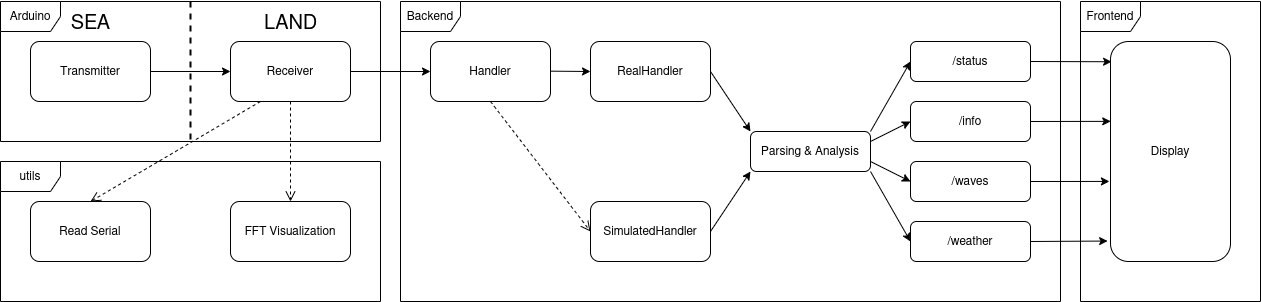
\includegraphics[width=1\linewidth]{assets/workflow.png}
        \caption{Workflow}
        \label{fig:enter-label}
    \end{figure}

\newpage
\section{Arduino}
In this section, we discuss the Arduino system’s features, capabilities, and architecture. The role of the Arduino module is to acquire raw data from multiple sensors, process and format it into structured packets, and wirelessly transmit it to the receiver for further handling. This hardware platform serves as the primary interface with the physical environment, enabling real-time environmental monitoring and data collection.
\subsection{Hardware Components}
    \subsubsection{Sensor Selection}
    We aimed to develop a compact and cost-effective environmental sensing system capable of monitoring atmospheric conditions, motion dynamics, and geographic positioning. This is the reason why the following three sensors were integrated into the transmitter node:
    
    \begin{tabular}{@{}m{0.25\textwidth} m{0.7\textwidth}@{}}
        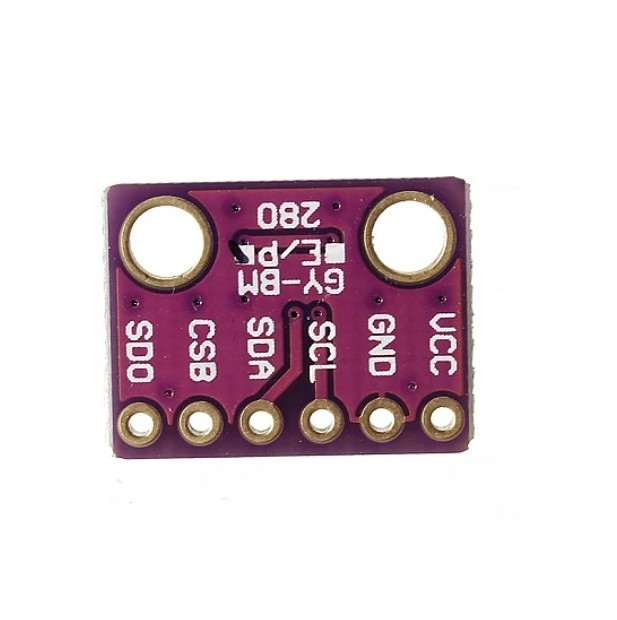
\includegraphics[width=0.9\linewidth, angle=90]{assets/bmp280.jpg} &
        \textbf{BMP280}: Measures atmospheric temperature and pressure with high precision and stability. \\
        
        \hspace{7mm} 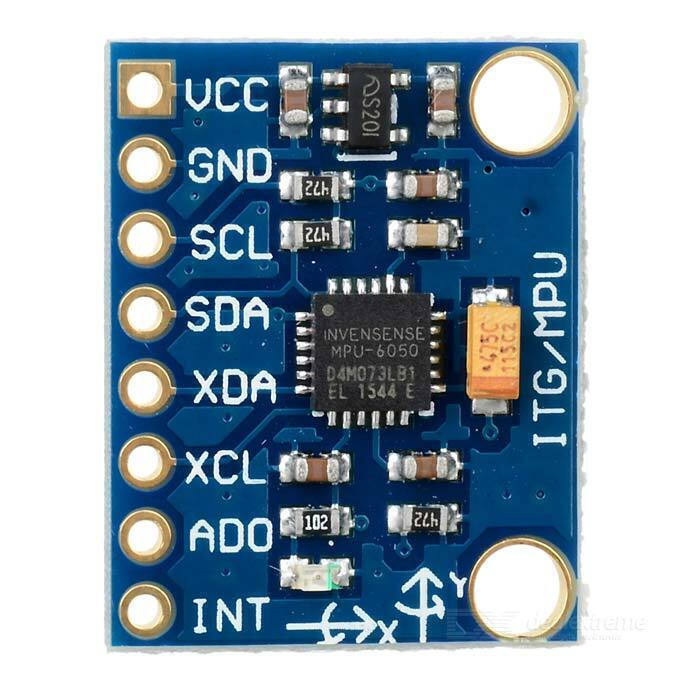
\includegraphics[width=0.6\linewidth]{assets/mpu6050.jpeg} &
        \textbf{MPU6050}: A 6-axis accelerometer and gyroscope used to estimate wave impact or surface motion dynamics (via the z-axis). \\
        
        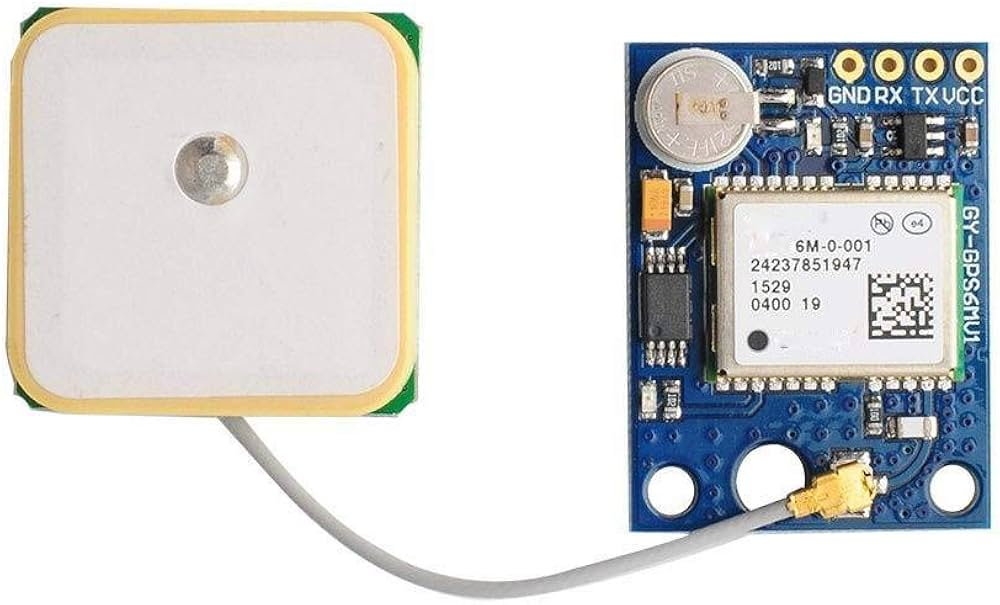
\includegraphics[width=0.9\linewidth]{assets/neo_6M_gps.jpg} &
        \textbf{NEO-6M}: A GPS module, known for its compact size, affordability and reliable performance. \\
    \end{tabular}
    
    These sensors were selected for their balance between accuracy, affordability and compatibility with Arduino-based systems.
    
    \subsubsection{Wiring and Pinout}
    \begin{itemize}
        \item \textbf{BMP280} is connected via I\textsuperscript{2}C using default SDA and SCL pins.
        \item \textbf{MPU6050} shares the same I\textsuperscript{2}C bus.
        \item \textbf{NEO-6M} is connected via UART using digital pin 2 and 3 for the Rx and Tx connections respectively.
        \item \textbf{RF22 module} uses SPI, with connections depending on the specific Arduino board used (for the Uno: MOSI = 11, MISO = 12, SCK = 13, SS = 10).
    \end{itemize}
    
    \begin{figure} [h]
            \centering
            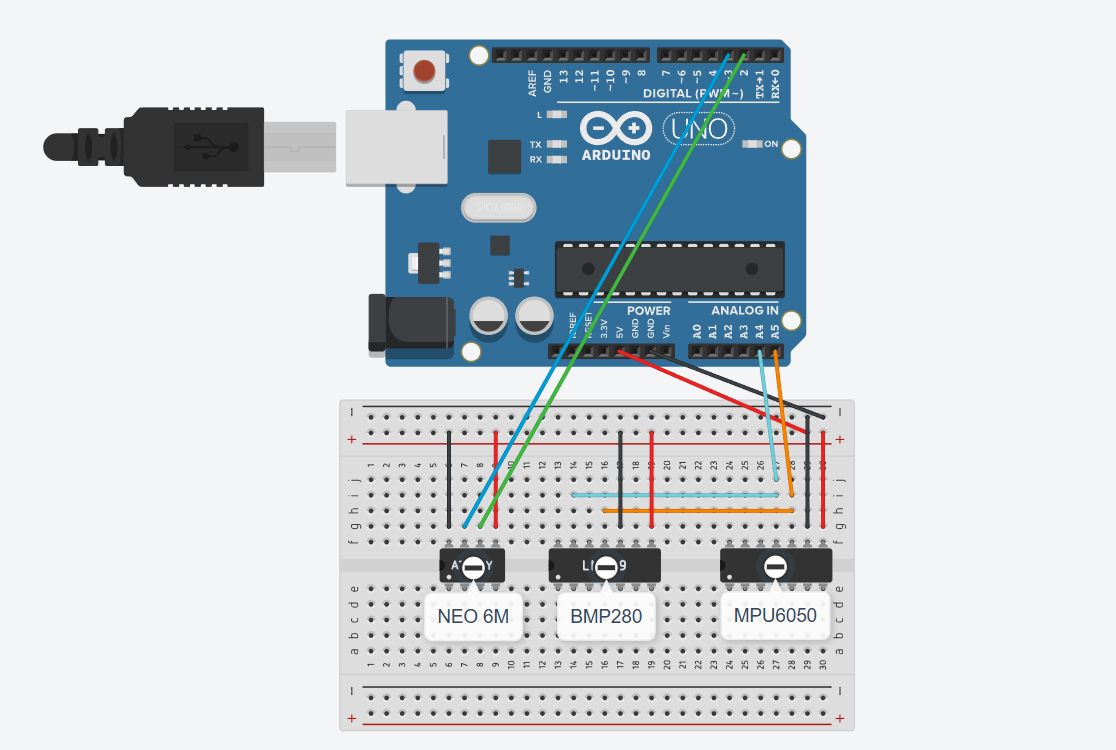
\includegraphics[width=0.5\linewidth]{assets/circuit-design.png}
            \caption{Circuit Design}
            \label{fig:enter-label}
    \end{figure}
    \newpage
    
    \subsubsection{Enclosure and Mounting}
    The enclosure is waterproof and weather resistant, as well as plastic, so that the various transmissions can pass uninterrupted. The MPU6050 sensor is oriented such that the z-axis faces upwards, enabling detection of vertical movement from wave activity.
    
\subsection{Transmitter Module}
    \subsubsection{Data Acquisition Loop}
    Sensor readings are acquired in each loop iteration:
    \begin{itemize}
        \item BMP280 returns temperature and pressure.
        \item MPU6050 returns raw acceleration and gyroscopic values.
        \item NEO-6M returns latitude and longitude.
    \end{itemize}
    Every second, a full data packet is composed, including coordinates, temperature, pressure, signal strength and vertical acceleration. In intermediate cycles, only acceleration data are transmitted to reduce energy consumption.
    
    \subsubsection{Transmission}
    Communication is carried out using RF22 modules configured with GFSK modulation at 440 MHz. Packets are transmitted using the sendtoWait() function, which includes acknowledgment. The configuration is set to use the maximum transmission power of 20 dBm, with modulation settings optimized to balance range and speed.
    
    \subsubsection{Power Management}
    Although advanced sleep modes are not implemented, energy efficiency is improved through selective data transmission (with full packets sent once per second), configurable transmission power, and the use of power-efficient sensors.
    
\subsection{Receiver Module}
    \subsubsection{Reception}
    The receiver node mirrors the transmitter's configuration for compatibility. It uses the same frequency and modulation settings, continuously listens for incoming data packets using the \texttt{recvfromAck()} function, and calculates the signal strength (RSSI) for logging and diagnostics.
    
    \subsubsection{Serial Output}
    Incoming data packets are printed directly onto the serial monitor in string format. This output is redirected to the backend and later to the GUI for end-user visualization and analysis.

\newpage
\section{Backend}
In this section we discuss the backend's features and capabilities, as well as its architecture. The role of the backend is to capture raw data from the sensor, analyze it, package it and send it to the frontend to be displayed in a meaningful way.

\subsection{Data Ingestion}
The data ingestion system is designed with a flexible architecture that accommodates both development and production environments through two specialized handlers; \texttt{SimulatedHandler} and \texttt{RealHandler}. Both handlers expose a consistent interface through the \texttt{SerialHandler} facade, which transparently selects the appropriate implementation based on the configured operational mode (\texttt{DEMO} or \texttt{DEPLOY}). This design pattern enables the application to operate identically regardless of data source, facilitating a smooth transition between development and production environments.

    \subsubsection{Simulated Handler}
    The \texttt{SimulatedHandler} provides a simulation environment for development and testing purposes. It generates realistic sensor data that mimics actual hardware outputs. The simulation incorporates deliberate variability -employing sinusoidal patterns with randomized amplitude, frequency and noise components- to realistically model sensor behavior. Data generation occurs in a dedicated thread running at 100Hz, maintaining a rolling buffer of 500 samples (equivalent to 5 seconds of historical acceleration data). This approach enabled us to test data processing pipelines, visualization systems and analytical algorithms without requiring physical sensor hardware.
    
    \subsubsection{Real Handler}
    The \texttt{RealHandler} establishes and maintains communication with physical Arduino-based sensor hardware via serial connection. It implements several resilience features including connection retry logic with exponential backoff, error handling for disconnection scenarios and automatic reconnection attempts. The handler continuously reads and parses incoming serial data through a dedicated thread, transforming raw string input into structured data objects according to the expected protocol format. Invalid or corrupted data is filtered through parsing logic that validates ranges and formats. Similar to its simulated counterpart, this handler maintains a time-series buffer of recent acceleration readings, enabling applications to analyze trends and patterns in the most recent sensor data.
    
    \begin{figure} [h]
        \centering
        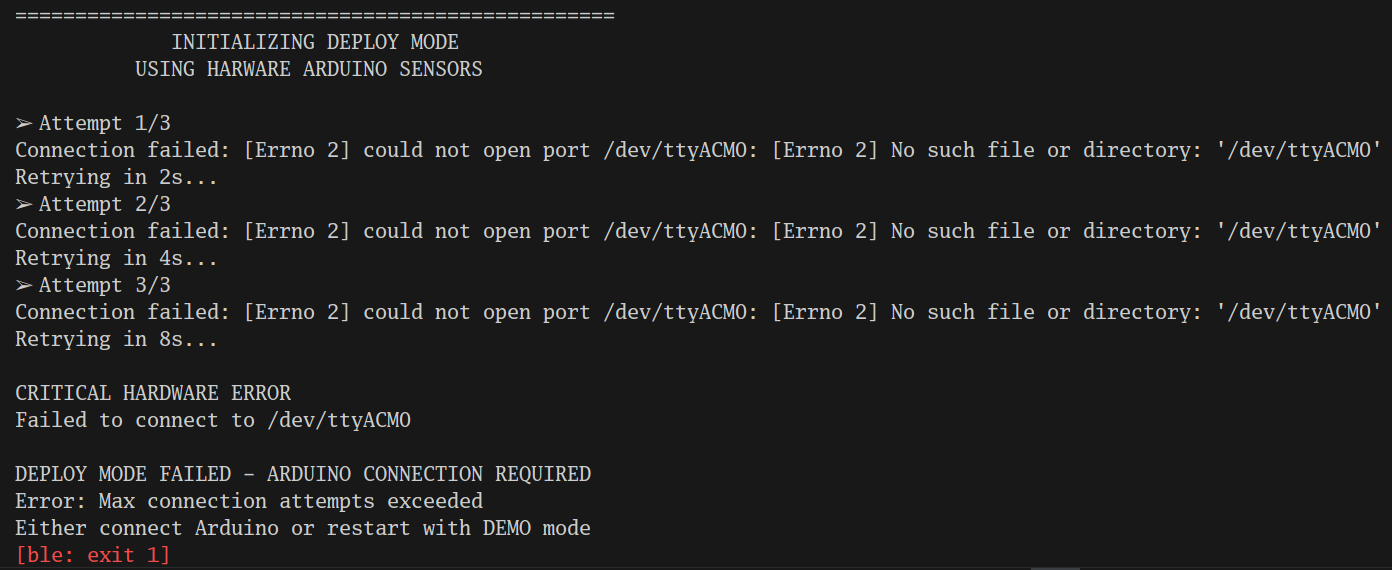
\includegraphics[width=0.75\linewidth]{assets/RealHandler.png}
        \caption{RealHandler Resilience}
        \label{fig:enter-label}
    \end{figure}

\subsection{Data Processing}

    \subsubsection{Wave Analysis}
    The wave analysis module implements a frequency-domain approach to extract meaningful metrics from raw accelerometer data. It performs Fast Fourier Transform (FFT) to identify the dominant wave frequency, filtering out low-frequency components (below 0.1 Hz) to eliminate sensor drift and environmental noise. The system converts raw accelerometer readings from LSB units to standard m/s² using a calibration factor derived from the MPU6050 sensor's sensitivity at ±2g range (datasheet). A physics-based heuristic transforms the acceleration variance into estimated wave height by applying appropriate scaling based on wave frequency, yielding actionable metrics that describe sea state conditions.

    \subsubsection{Mathematical Background}
    The shore impact analysis implements established coastal engineering models to translate wave metrics into practical inundation forecasts \cite{stockdon2006}. The system calculates fundamental wave parameters including period (reciprocal of frequency) and deep-water wavelength using standard gravity-based equations. The core of the analysis employs the Iribarren number (surf similarity parameter) to classify wave behavior as either dissipative or reflective/intermediate, applying the appropriate runup estimation formula for each regime. The model classifies hazard zones based on runup thresholds, with values exceeding 0.9 meters designated as high-risk (VE zone) \cite{fema2022}. The final inundation distance is calculated by applying the slope correction factor, providing horizontal reach estimates critical for coastal planning.

\subsection{API Endpoints}
In this section we analyze the API endpoints available for the frontend to call

    \subsubsection{Status}
    The /status endpoint provides essential system telemetry for monitoring the operational state of the device. It returns a JSON payload containing connectivity status, power information (battery percentage), and geolocation coordinates derived from the sensor data stream. The endpoint also includes signal strength metrics (measured in dBm) to facilitate deployment troubleshooting and network quality assessment. By serving as a lightweight health check, this endpoint enables rapid verification of device functionality without interrogating the more resource-intensive data processing pipelines.

    \subsubsection{Info}
    The /info endpoint exposes environmental context data captured by the sensor array, specifically temperature (in degrees Celsius) and barometric pressure (in hectopascals).

    \subsubsection{Waves}
    The /waves endpoint delivers processed wave characteristics and their projected coastal impact. It retrieves the acceleration time-series buffer from the sensor handler and passes it through the wave analysis pipeline to extract frequency and height parameters. These metrics are then fed into the shore impact model to calculate vertical runup height, FEMA flood zone classification and horizontal inundation distance based on a predefined slope parameter (set to 0.05 const). This endpoint represents the system's primary analytical output, transforming raw sensor data into actionable coastal flooding information delivered in a standardized JSON format.

    \subsubsection{Weather}
    The /weather endpoint enriches the system's data with third-party meteorological information by interfacing with the OpenWeatherMap API. It dynamically constructs API requests using the device's current geolocation coordinates and securely transmits the authentication key from environment variables. The endpoint parses the response to extract wind parameters (speed and direction) along with general weather conditions and human-readable descriptions.

\subsection{Test Functions and Utilities}
    \subsubsection{Package Check}
    The package check utility verifies that all dependencies meet the required version specifications, preventing compatibility issues. It generates a formatted tabular output with clear visual indicators for each package's status: successfully meeting requirements (✅), outdated versions requiring updates (❌ Too Old), or missing packages that need installation (❌ Not Found).
    
    \begin{figure} [h]
        \centering
        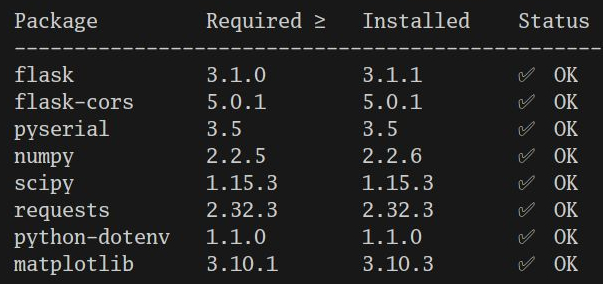
\includegraphics[width=0.5\linewidth]{assets/check-packages.png}
        \caption{Package Check}
        \label{fig:enter-label}
    \end{figure}
    
    \subsubsection{Serial Screening}
    The serial screening utility provides direct access to the raw data stream from connected Arduino hardware, bypassing the application's processing pipelines. It establishes a serial connection to the configured port using the same parameters as the main application (9600 baud) and continuously reads, parses and displays each data frame in real-time. This tool was particularly useful during initial deployment to confirm proper hardware operation before launching the complete application stack.

    \subsubsection{FFT Visualization}
    The FFT visualization tool enables detailed analysis of sensor data characteristics through both time and frequency domain representations. It captures a configurable duration of acceleration data (default 30 seconds) using the same SerialHandler interface as the main application, ensuring consistency between visualization and production operation. The tool produces a dual-panel plot showing raw acceleration values (in m/s²) against time in the upper panel and the corresponding frequency spectrum via Fast Fourier Transform in the lower panel. The visualization highlights the detected dominant frequency with a vertical marker. This dual representation allowed us to correlate time-domain patterns with their frequency components, aiding in algorithm refinement and system tuning.

    \begin{figure} [h]
        \centering
        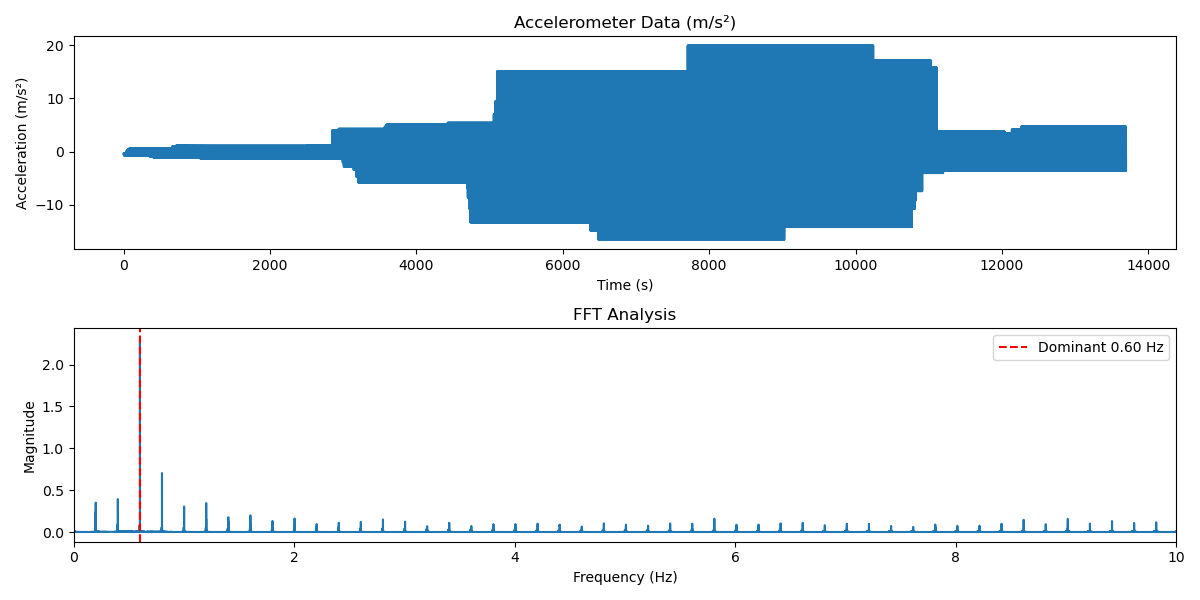
\includegraphics[width=1\linewidth]{assets/fft_visualization.png}
        \caption{FFT Visualization}
        \label{fig:enter-label}
    \end{figure}

    \subsubsection{Cleaning}
    The cleaning utility implements system maintenance functionality through a shell script that removes Python cache files. This utility improves development workflow by preventing stale bytecode from causing unexpected behavior after code changes, particularly when performing major refactoring.

\section{Frontend}
This section focuses on explaining the part of the project that is responsible for visualizing the data we gathered in real-time and making it accessible to the public through a web application.
\subsection{Tools and Frameworks Used}
    The application is built using several different tools and frameworks with the goal to create a modern and intuitive user experience. In more depth, we used \textbf{React} along with \textbf{TypeScript}, which serves as the foundation for the component-based architecture that we used, providing a responsive and interactive user interface, making it feel closer to a native application instead of a traditional website. TypeScript is used to add static typing, in order to enhance code reliability, readability as well as maintainability. We also used several libraries for enchancing the user experience, like:
    \begin{itemize}
        \item \textbf{Recharts}: Powers the data visualization for the wave height monitoring with interactive charts
        \item \textbf{Lucide React}: Supplies the iconography used throughout the interface for weather conditions, status indicators, and UI elements
        \item \textbf{Framer Motion}: Provides fluid animations and transitions for alerts and UI elements
        \item \textbf{Tailwind CSS}: Implements custom styling with utility-first classes, creating consistent design patterns across components
    \end{itemize}
    This technology stack creates a fast, responsive application capable of handling real-time data visualization with minimal development overhead.
        
\subsection{Look and Feel}
    The application follows a modern weather dashboard aesthetic with several notable design choices.
    \begin{figure}[h]
        \centering
        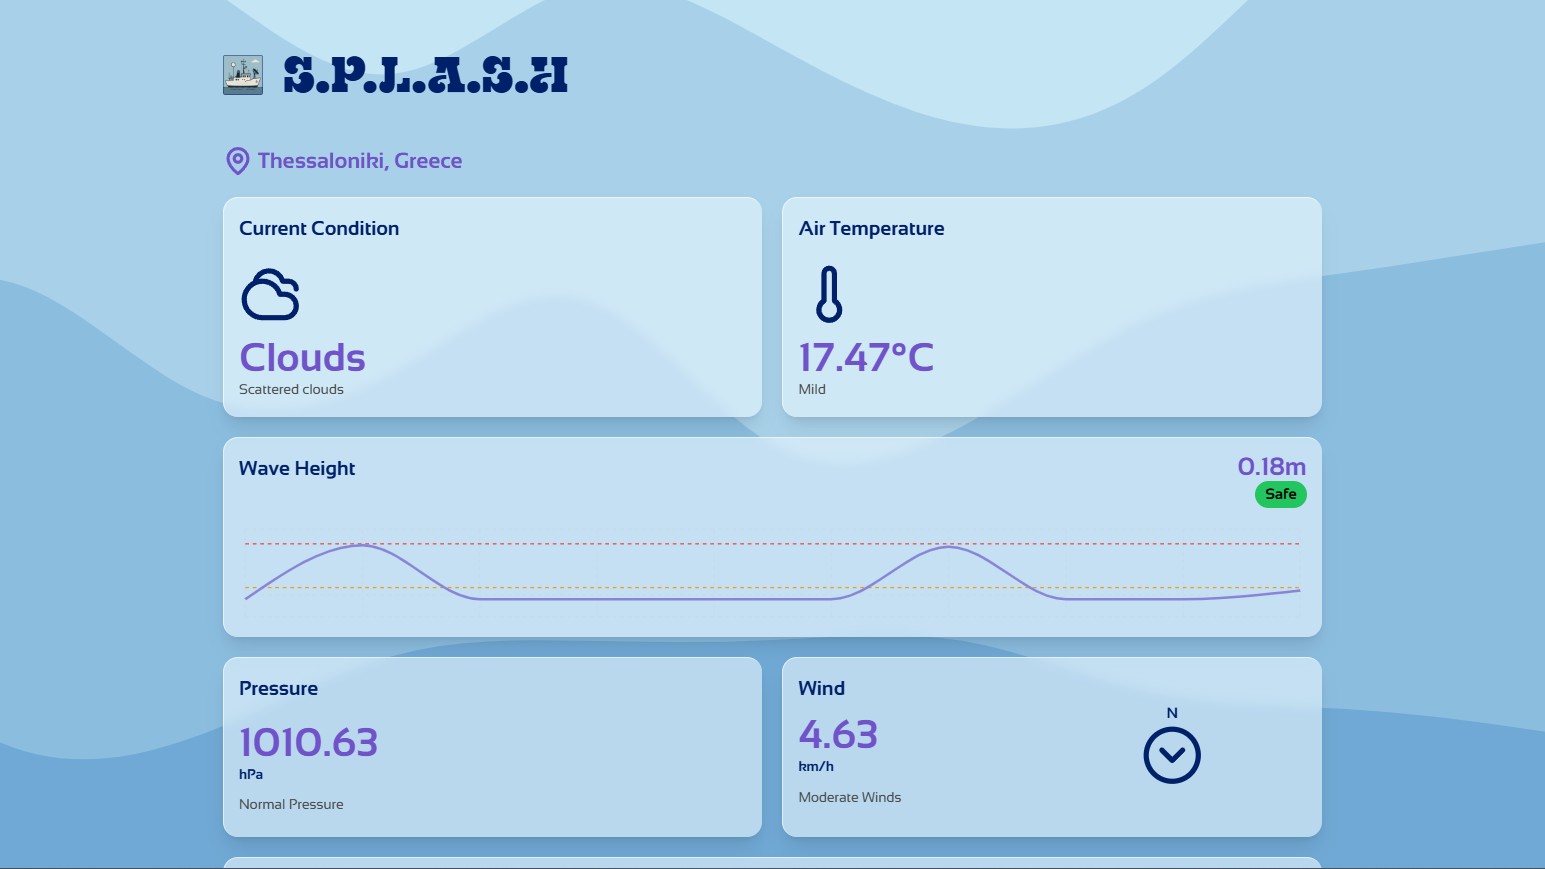
\includegraphics[width=1\linewidth]{assets/FE_F2.png}
        \caption{Web application look}
        \label{fig:frontend}
    \end{figure}
    \\
    More specifically, the website follows a \textit{Glassmorphic} design inspired by popular weather websites, making it easy and familiar for the user to understand the data shown.
    \subsubsection{Component Based Design}
    The website used native widgets to display information. Each widget is has a title, explaining to the user what it shows and also gives descriptions for what the data translates to in the real world (i.e. comments if current pressure is above or below average). Widgets like \textit{Current Condition} and \textit{Wind} also have dynamic icons that change in accordance to the conditions that it shows. The widgets that are currently available to our application are:
    \begin{itemize}
        \item The \textit{Current Condition} widget, which changes it's icon as well as color if the weather is \textit{Cloudy}, \textit{Raining} or \textit{Sunny}
        \item The \textit{Air Temperature} widget, that displays the current temperature as measured from the drone's on board sensor
        \item The \textit{Pressure} widget, showing the atmospheric pressure as measured from the drone's on board sensor
        \item The \textit{Wind} widget, showing a 'compass' icon along with the wind speed, that changes to the actual direction of the wind at the location of our drone.
        \item The \textit{Avg Dist to Shore} widget, displaying the projected distance that the average wave will reach to the shore
        \item The \textit{Drone Status} widget, giving valuable information about the drone itself, like battery and signal strength status
        \item The \textit{Wave Height} widget, shows the actual height of the wave from sea level as well as a chart of the last 10 values, making the information more readable and useful to the user, giving a sense of scale to each measurement.
    \end{itemize}
    This design philosophy allows us to easily add new widgets to our application on future updates making it modular while keeping a modern look.

    \subsubsection{Notifications and Warnings}
    The web application also has the ability to notify the user with alerts regarding extreme weather events or other events regarding the status of the drone.
    More specifically these notifications are categorized based on their priority:
    \begin{itemize}
        \item \textbf{Low priority}: At its current state, low priority notifications may be for example low signal strength or if the application fails to connect with a backend server
        \item \textbf{High priority}: The notifications warn the user for possible extreme weather events, like a tsunami in the case that a abnormally high wave appears
    \end{itemize}
    Low priority notifications are indicated with a \textit{yellow} color, while high priority notifications are showed in \textit{red}.
    
    \begin{figure}[h]
        \centering
        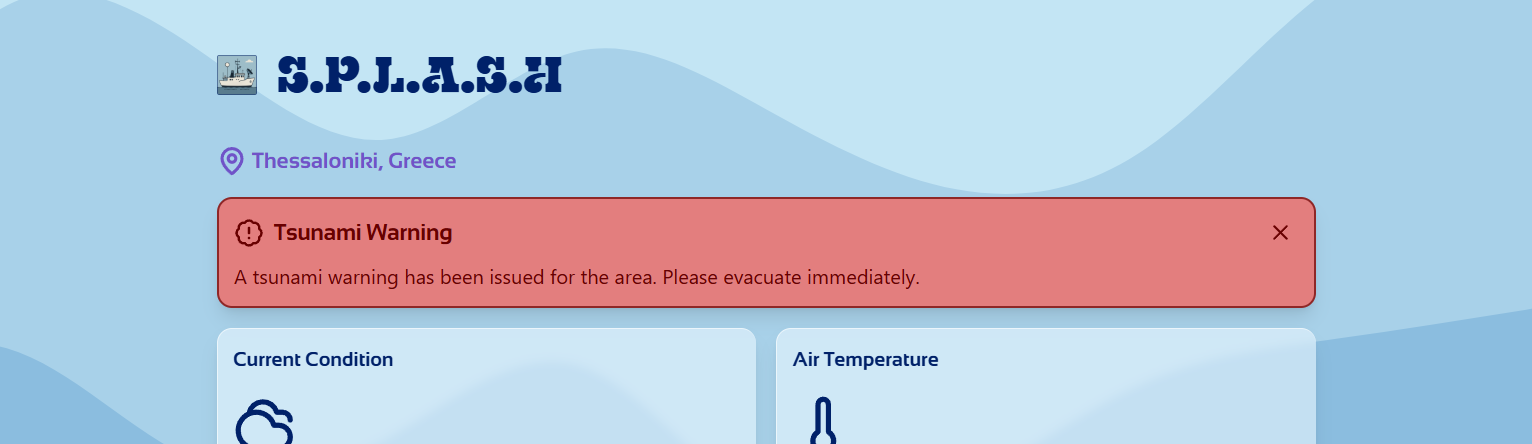
\includegraphics[width=0.75\linewidth]{assets/FE_F1.png}\\
        \vspace{1cm}
        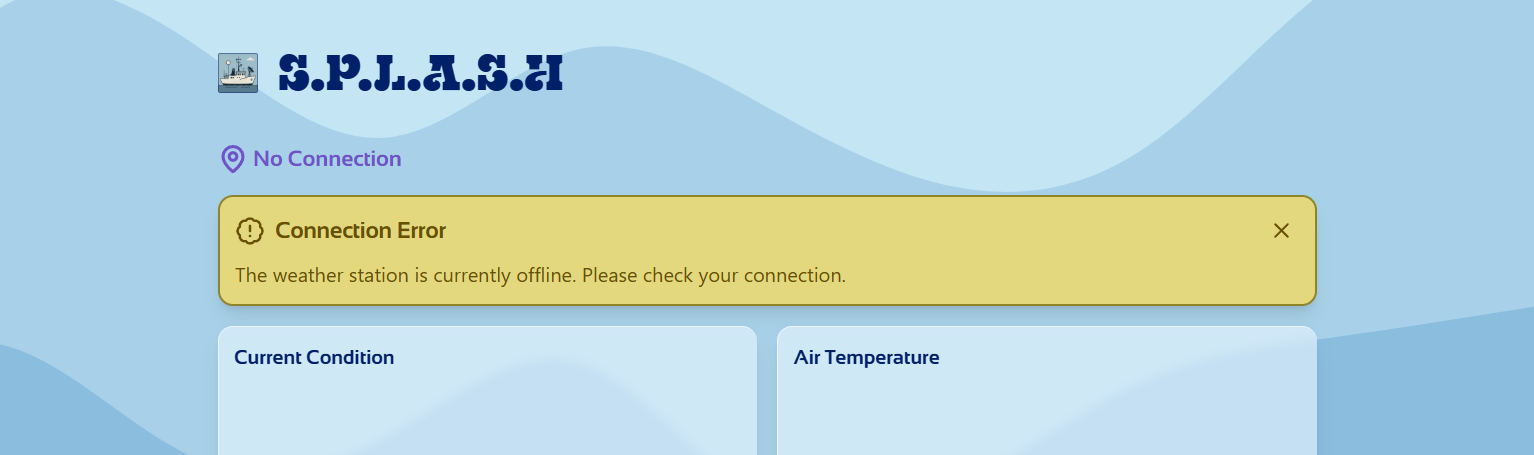
\includegraphics[width=0.75\linewidth]{assets/FE_F4.png}
        \caption{Notifications}
        \label{fig:notifications}
    \end{figure}
    
\subsection{Data API Integration}
    \subsubsection{API Requests}
    Each widget handles API requests independently. Different widgets fetch data at different time intervals. This approach, while it isn't the most efficient when making API calls, makes the system more modular when creating new widgets and expanding the functionality of the application. More specifically:
    \begin{itemize}
        \item The \textit{Current Condition} and \textit{Wind} widgets, make API requests to the backend server every \textit{3} minutes. This is done because our current approach relies on an external API for collecting this data, and there is a limit to the number of requests the system can make daily.
        \item The \textit{Wave Height} widget, makes request to our backend request every second, as this makes its corresponding graph more responsive and informative
        \item The rest of the widgets currently implemented, have intervals set at \textit{30} seconds, as they do not rely on any external APIs and don't overload our backend server
    \end{itemize}
    Lastly, low as well as high priority alerts have requests interval set at \textit{10} seconds, ensuring that notifications can arrive to the user in time.
    
    \subsubsection{Simulated and Live Modes}
    Considering the difficulties associated with setting up a drone and backend infrastructure for a live demo, we have also set up the ability for the user to test our application with the help of an always online backend server, providing the frontend with simulated data. This setting can be changed any time at the bottom of the main page. If the user wants to test a real implementation of our project, they can do so, be pressing the 'Live' button, and filling in the IP and port number of their backend server.
    
    \begin{figure}[H]
        \centering
        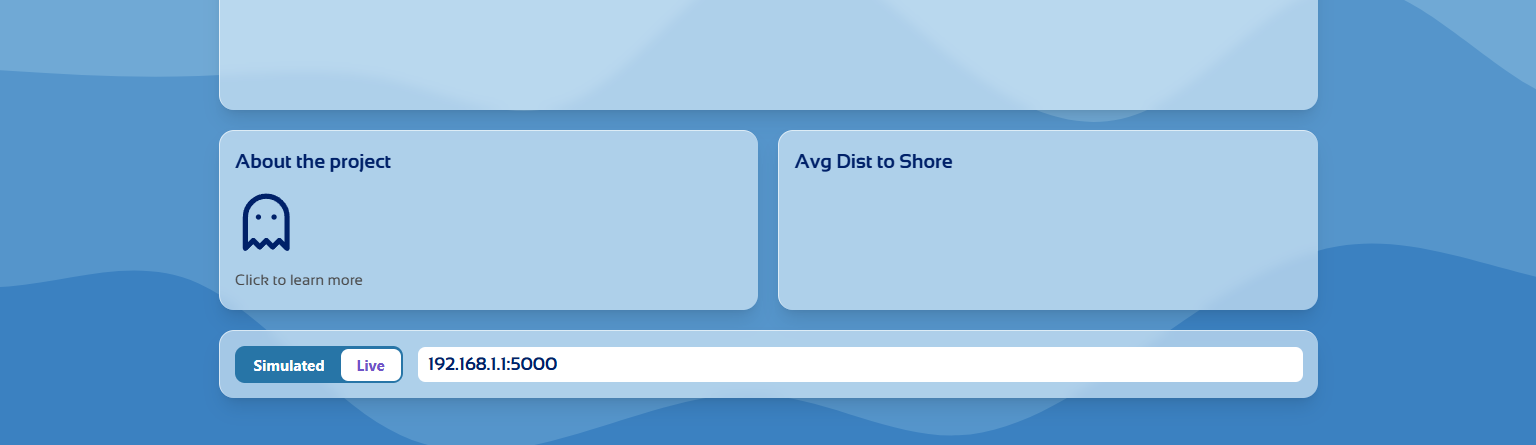
\includegraphics[width=1\linewidth]{assets/FE_F5.png}
        \caption{Live/Simulated Mode}
        \label{fig:simulated}
    \end{figure}

\newpage
\section{Conclusions}
    \subsection{Summary of Achievements}

    The \textit{SPLASH} project successfully delivers a functional, low-cost and modular system for real-time maritime environmental monitoring. 
    
    A fully operational Arduino-based transmitter node was designed, integrating BMP280, MPU6050 and NEO-6M sensors to capture temperature, atmospheric pressure, vertical acceleration and geolocation data. Wireless communication was established using RF22 modules operating at 440 MHz with GFSK modulation, enabling efficient and reliable data transfer between the transmitter and receiver.
    
    The backend system supports both simulated and real-time sensor data ingestion. It features a resilient serial communication handler, error recovery mechanisms and a rolling time-series buffer for acceleration data. Data processing includes an FFT-based wave analysis module capable of estimating dominant wave frequency and height. This was further extended with a physics-based model to compute coastal impact metrics and classify flood risk zones.
    
    In addition to the core system, a range of supporting tools was developed, including utilities for serial data inspection, FFT visualization, dependency checking and codebase cleaning. The overall architecture emphasized modularity, allowing for easy expansion with additional sensors, backend features, or frontend components in the future.
    
    A set of API endpoints was created to expose system data, including status, environmental conditions, wave characteristics and third-party weather information. These endpoints formed the foundation for a frontend web application. The frontend employed a modern glassmorphic design and interactive widgets to visualize data in real time, supporting both simulated and live data modes.
    
    This set of accomplishments demonstrates the successful implementation of a scalable and user-friendly system for coastal monitoring.
    
    \subsection{Lessons Learned}
    Through the implementation of this project, we gained valuable experience in building a cyber-physical system and became more adept at capturing, interpreting, and analyzing sensor data. Our programming and engineering skills improved significantly as we tackled challenges such as setting up a backend web server, developing a modular API architecture, and crafting both the physical prototype and a waterproof enclosure. We also deepened our understanding of wireless communication, sensor integration, and data visualization. This project provided us with a comprehensive, hands-on opportunity to bridge hardware with software and deliver meaningful environmental insights through a full-stack solution.
    \subsection{Future Work}
    Future improvements to the system may include:
    \begin{itemize}
        \item Implementing a mesh network of drones for wider coverage and resilience
        \item Integrating additional environmental sensors (e.g., humidity)
        \item Embedding the hardware into a single hydrodynamic boat
        \item Developing an automated navigation and docking system
        \item Utilizing solar power for energy autonomy
        \item Adding proper battery level monitoring to the \texttt{/status} endpoint
    \end{itemize}

\newpage
\appendix
\section{User Manual}
How to operate \textit{SPLASH}:
\begin{itemize}
    \item Power on the Arduino-based sensor module
    \item Ensure the receiver is connected to a computer and listening via serial
    \item Launch the backend server
    \item Open the web application to view real-time data
\end{itemize}

\section{Bill of Materials}

This is a \textit{rough} estimation of the total cost of the project.
\renewcommand{\arraystretch}{1.3}
\begin{table}[H]
    \centering
    \begin{tabular}{@{} C C C @{}}
        \toprule
        \multicolumn{1}{c}{\textbf{Item}} 
            & \multicolumn{1}{c}{\textbf{Quantity}} 
            & \multicolumn{1}{c}{\textbf{Price (€)}} \\
        \midrule
        Arduino Uno R3           & 2  & 25  \\
        RF22 card                & 2  & 32  \\
        Waterproof enclosure     & 1  & 22  \\
        Powerbank                & 1  & 10  \\
        NEO-6M GPS               & 1  &  7  \\
        MPU6050 Sensor           & 1  &  3  \\
        BMP280 Sensor            & 1  &  2  \\
        USB Power Cable          & 1  &  1  \\
        Jumper Wires             & 10 & 0.1 \\
        Prototyping board        & 1  & .5  \\
        \midrule
        \textbf{Total}           &   & \textbf{160.5} \\
        \bottomrule
    \end{tabular}
    \caption{Bill of Materials}
    \label{tab:bom}
\end{table}

\section{Tools and Frameworks}
The following tools and frameworks were used:
\begin{itemize}
  \item Arduino IDE (Sensor Interaction)
  \item Python with Flask (Backend API)
  \item TypeScript with React (Frontend UI)
\end{itemize}

\begin{thebibliography}{9}
    \bibitem[\href{https://data-ww3.ifremer.fr/BIB/Stockdon_etal_CE2006.pdf}{1}]{stockdon2006}
        Stockdon, H.~F.; Holman, R.~A.; Reichmuth, A.; Van Ormondt, M.  
        Estimation of shoreline position and change using airborne LiDAR data.  
    \emph{Coastal Engineering} \textbf{53}(3), 2006.
    \bibitem[\href{https://www.fema.gov/sites/default/files/documents/fema_coastal-floodplain-mapping_112022.pdf}{2}]{fema2022}
        Federal Emergency Management Agency (FEMA).  
        Coastal Floodplain Mapping Report. November 2022.
\end{thebibliography}

\end{document}